\documentclass{minimal}
\usepackage{tikz}
\usepackage{palatino}
\renewcommand{\familydefault}{\sfdefault}

\usetikzlibrary{calc,trees,positioning,arrows,chains,shapes.geometric,%
decorations.pathreplacing,decorations.pathmorphing,shapes,%
matrix,shapes.symbols}

\tikzset{
>=stealth',
punktchain/.style={ rectangle, rounded corners, draw=black, very thick, text width=10em, minimum height=3em, text centered, on chain},
statement/.style={ circle, draw=black, text width=0em, minimum height=0em, text centered},
line/.style={draw, thick, ->},
merge/.style={draw, thick, -},
element/.style={ tape, top color=white, bottom color=blue!50!black!60!, minimum width=8em, draw=blue!40!black!90, very thick, text width=10em, minimum height=3.5em, text centered, on chain},
every join/.style={->, thick,shorten >=1pt},
decoration={brace},
tuborg/.style={decorate},
tubnode/.style={midway, right=2pt, text width=6cm},
}
\begin{document}
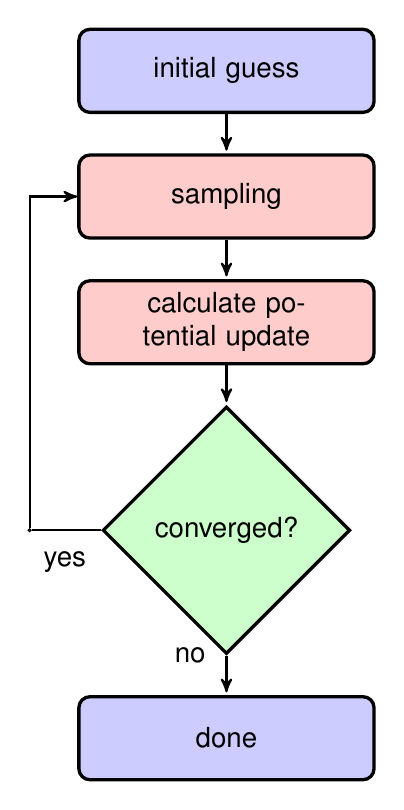
\begin{tikzpicture}
[node distance=.5cm, start chain=going below,]

\node[punktchain, join, fill=blue!20] (init_global) {initial guess};
%\draw[tuborg, decoration={brace}] let \p1=(init_global.north), \p2=(init_global.south) in
%($(2, \y1)$) -- ($(2, \y2)$) node[tubnode] {Initialize global variables (paths to scripts, executables and user-defined scripts) };

%\node[punktchain, join, fill=blue!20] (init_step) {sampling};
%\draw[tuborg, decoration={brace}] let \p1=(init_step.north), \p2=(init_step.south) in ($(2, \y1)$) -- ($(2, \y2)$) node[tubnode] {Convert target distribution functions into internal format, prepare input files, copy data of the previous step};

\node[punktchain, join, fill=red!20] (sampling) {sampling};
%\draw[tuborg, decoration={brace}] let \p1=(sampling.north), \p2=(sampling.south) in
%    ($(2, \y1)$) -- ($(2, \y2)$) node[tubnode] {Canonical ensemble sampling with molecular dynamics, stochastic dynamics or Monte Carlo techniques};

\node[punktchain, join, fill=red!20] (pot_update) {calculate potential update};
%\draw[tuborg, decoration={brace}] let \p1=(pot_update.north), \p2=(pot_update.south) in
%($(2, \y1)$) -- ($(2, \y2)$) node[tubnode, text width=6cm] {Analysis of the run. Evaluation of distribution functions, potential updates $\Delta U^{(n)}$ };

\tikzstyle{decision} = [diamond, draw = black, very thick, %fill=blue!20,
  text width=8em, on chain, text badly centered, node distance=4cm, inner sep=0pt]

\node [decision, join, fill=green!20] (continue) {converged?};
%\draw[tuborg, decoration={brace}] let \p1=(continue.north), \p2=(continue.south) in
%    ($(2, \y1)$) -- ($(2, \y2)$) node[tubnode, text width=6cm]
%    {   Evaluation of the convergence criterion either for $\Delta U^{(n)}$ or distribution functions. Check the number of iterations.};

\node[punktchain, join, fill=blue!20] (end) {done};

\node[statement, left of=continue, node distance=2.5cm, inner sep=0pt ] (positive) {};

\path [merge] (continue.west) |- (positive.east);
\path [line] (positive.north) |- (sampling.west);

\node[anchor=north] (a) at ([xshift=12pt, yshift=-4pt] positive.east) {yes};
\node[anchor=east] (b) at ([xshift=-4pt] continue.south) {no};

\end{tikzpicture}
\end{document}
